\section{A Refined View of Assurances} \label{sec:synthesis}
    From the review of Quadrants I. through IV. of the formal/informal, explicit/implicit plane (see figure \ref{fig:trust_assurance_intention}), we are able to find some insights with respect to assurances and can discuss them in a more comprehensive way. Using the surveyed papers as a guide, a more detailed look at the path from the AIA to the User can be constructed. Figure \ref{fig:assurance_path} shows some of the key steps between an AIA source capability, and a user trust target.

    \begin{figure}[htbp]
        \centering
        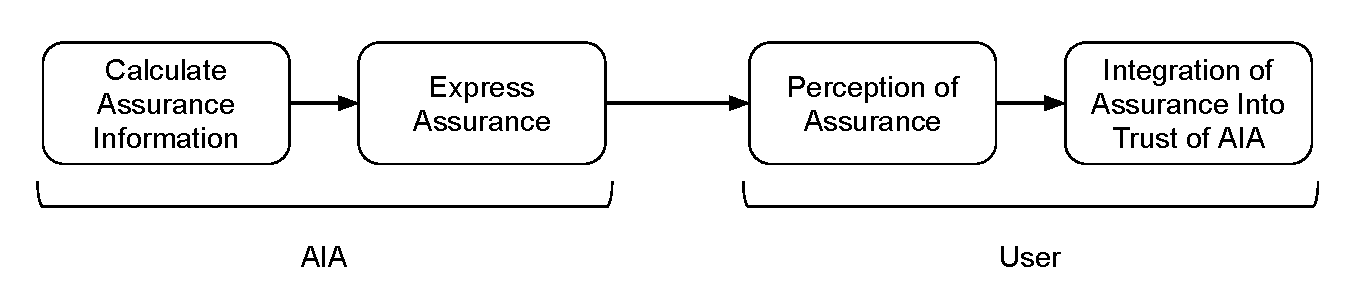
\includegraphics[width=0.9\textwidth]{Figures/Assurance_Path.pdf}
        \caption{More detailed steps involved in giving and receiving assurances}
        \label{fig:assurance_path}
    \end{figure}

    \subsection{Considering the User in Designing Assurances} \label{sec:consider_human}
    In a relationship between a human and an AIA the human user will have TRBs. In general the human user will not have knowledge regarding what assurances are implicit or explicit. It is critical to note that in the absence of explicit assurances the human will instead use implicit assurances to inform their TRBs.

    As a simple example, in \cite{Muir1994-ow} a simple flow-rate is provided to the user, they then created a mental model of the reliability of the AIA to inform their TRBs. Creating this mental model takes time, and the model is prone to cognitive biases (discussed a bit more below).

    To the user all assurances are the same, that is to say that any property or behavior of an AIA that affects trust is an assurance, and that it doesn't matter whether the assurance was designed or not (is explicit or implicit). As illustrated in Figure \ref{fig:assurance_path}, perception of the assurance is the first step in which the human user is involved (the two previous steps belong to the AIA). This highlights the idea that human perception (both sensory and cognitive) needs to be taken into account when designing assurances.

\subsubsection{Perception of Assurance}
    An important consideration when designing assurances is whether a human can perceive the assurances being given. If so, to what extent is the information from the assurance transfered (i.e. how much information was lost in the communication)? A few examples include: an AIA giving an auditory assurance in a noisy room and the user not hearing it, or an AIA displaying an assurance to a user that has obstructed vision.

    What perceptions are beneficial to a certain task? Looking at \cite{Dragan2013-wd} and \cite{Wu2016-ei} shows that sometimes the same technique can have different effects. In \cite{Dragan2013-wd} the AIA is made more trustworthy by making the motions more human-like, whereas in \cite{Wu2016-ei} making the AIA more human-like resulted in a decrease of trustworthiness. This highlights the need to understand the environment in which the AIA and human will interact, and to modify assurances appropriately based on desirable perceptions.
    
    A second more nuanced point is whether the user can process the information received. This is perhaps most easily illustrated by considering a non-expert user who cannot understand highly technical assurances regarding the AIA. However, less trivial manifestations may be troubling. This point was not directly addressed in the survey papers, but evidence of its existence were seen. For example in quadrant I \cite{Riley1996-qm}, and \cite{Freedy2007-sg} both observed evidence of framing effects (or the tendency of humans to have biased trust based on the order in which they encountered AIA with different levels of competency). This suggests the existence of other kinds of typical cognitive behaviors such as recency effects (having biased trust based on recent experiences), that might affect the ability of a human user to. With these cognitive affects we see that the human brain inherently has limitations to being able to process assurances. These limitations must be considered when designing assurances.

\subsubsection{The Effects of Assurances on User Trust}
    When it comes time to measure the effect of assurances on a human's trust the surveyed literature uses two main approaches. The first is self-reported changes based on questionairres, the second involves measuring changes of user's TRBs. Evidence is presented in \cite{Dzindolet2003-ts} that illustrates that sometimes changes is self-reported trust do not result in changes in TRBs. As previously discussed, the goal of assurances are to elicit appropriate TRBs from the human user towards the AIA. From this perspective measuring changes in TRBs is the more objective approach to measure the effect of assurances. Attempting to measure the self-reported trust of a user has a couple of key weaknesses: First, measuring self-reported trust does not measure TRBs and thus misses the goal of assurances; second, gathering self-reported data is also subject to typical biases of different users, and may fluctuate from task to task for the same user. In view of these arguments we recommend that the effects of assurances be primarily measured through changes in TRBs, with self-reports being used as a secondary source of information.

    \subsection{Considering the AIA in Designing Assurances} \label{sec:consider_AIA}
\subsubsection{Calculating Assurances}
    In order to give an assurance an AIA must first be able to create one, or more specifically the AIA must be able to calculate the information that needs to be conveyed, this is a point seen when reading \cite{Kaniarasu2013-ho,Chen2014-dk}. This is currently a limitation of many AIAs that do not possess the ability to calculate assurances for their respective capabilities. AIAs must have the ability to be introspective (perform analysis on \emph{its own} functions, capabilities, and models, to compute assurances), as well as extrospective (perform analysis on the function, capabilities, and  models of \emph{external entities} to compute assurances). An AIA that possesses both together can be referred to as circumspective. Once circumspective analysis has occurred then the AIA must be able to express the assurances. This is a challenge that needs to be addressed directly, and the surveyed work (and other similar work) will help guide the development of those capabilities.

    To date several different promising methods have been used to calculate assurances in different applications. These include modifying the objective to consider a user's trust (i.e. legible motion \cite{Dragan2013-wd}, and safe learning), calculating intended actions, methods operating on POMDPs have also been developed in an attempt to quantify how they perform. Researchers from quadrant III and IV have developed many other promising approaches that involve predicting performance, making models more interpretable by simplifying them and/or adding structure, reducing the dimensionality, explaining the reasoning of decision making AIAs, and checking models, guaranteeing performance through V\&V, learning safely, dealing with non-stationary training/test data, and learning better features. Many of these methods are ready to be used in more formal human-AIA trust studies to verify their utility in this application.

    It is important to recognize the fact that AIAs may possess several different capabilities, and that each may be more or less trustworthy. This suggests that there must be several assurances created in order to assure the user with respect to each of the different capabilities. As discussed by \cite{Chen2014-dk} assurances from different capabilities may be more or less important depending on the situation (i.e. sometimes the user may need to understand why a decision was made, but not at other times).

\subsubsection{Expressing Assurances}
    An AIA must not only be able to calculate an assurance, but express it to the user as well. These expressions must be tailored to human strengths and weaknesses, some of which are mentioned in section \ref{sec:consider_human}. To state the point more bluntly, if an assurance is not expressed, or not perceived by the user, it is useless and has no effect. The expression of assurances to a human user is not a trivial topic and has been investigated mainly by those in quadrants I, and II by basic visualizations and natural language communication (and promising approaches like high dimensional visualization were mentioned in quadrants III and IV). There is, however, a body of research (not surveyed here) that considers how to communicate information to humans (i.e. as probabilities, or fractions, by text, or by plotting, etcetera). It is probable that marketing, and cognitive science have much to contribute to this topic. This research is critical in designing how to efficiently express assurances in a way that they will be perceived correctly by the user with the least possible information loss.

\subsubsection{The Imprecise Nature of Assurances}
    Due to the nature of trust (and humans in general), a single assurance might be targeted at influencing the competence dimension of trust, but it may also have effects on other dimensions. As an example an assurance that targets predictability may also have an affect on the probability of depending.

    Besides being difficult to separate effects on a single user, individual users are different as well. Thus no assurance will have an identical effect when given to two separate users. This makes it difficult to have precise effects on user trust behaviors.

    One might attempt to mitigate this uncertainty by using expressions that are more precise than others, such as displaying a probability distribution rather than on a maximum likelihood. This gets into some considerations about how the presentation of information affects the ability of a human to understand.


\subsection{Classes of Assurances}
    Given the considerations discussed above, we can make some attempt at classifying assurances.
    \subsubsection{Explicit and Implicit Assurances}
\citet{Sheridan1984-kx} briefly alluded to the existence of explicit and implicit assurances when they discussed the nature of how humans behave when working with automated systems. They suggested that the operator's perception of the automated system can be effected by `performance' and its `reports on its own performance'. 


\begin{description}
    \item [Explicit:] Assurances that are purposefully given to affect the trust of a user.
    \begin{itemize}
        \item Legible motion \cite{Dragan2013-wd}, which is motion calculated with the intent of being more understandable by a human
        \item $R^2$ value, gives some indication of how well the regression accounts for the variance of the data
    \end{itemize}
    \item [Implicit:] All other assurances that aren't explicit.
    \begin{itemize}
        \item Reliability in completing a task. Generally, the object of success is not to affect the user's trust (although this is a nice side-effect).
        \item The way an autonomous vehicle appears. For example something that looks neat will have a different effect on trust, than an AIA with wires dragging on the ground. 
    \end{itemize}
\end{description}



    \subsubsection{Source-Target Classification}
    It is convenient to refer to assurances by way of their source and target. Intuitively, there may be a set of different algorithms that are useful for making assurances that convey information about planning to the competence dimension of the user's trust. It is easier to refer to these assurances in terms of their source and target. So, for this example that class of algorithms would be the `planning-competence' class.
    
    Not only is this useful shorthand for communicating about the purpose of the algorithms, but it is useful in classifying the range of assurance algorithms that exist. There may also be a class of algorithms that span multiple source-target capabilities. For example there may be a kind of algorithm that can give a `learning-competence' assurance, as well as a `planning-competence' assurance.

    This is especially true since many of the AIA capabilities can overlap. Also, the effects of assurances cannot be guaranteed to affect only one trust dimension.

    Figure \ref{fig:Assurance_classes} shows the hierarchy of proposed assurance classes. The categories mirror those of the trust model proposed by \citet{McKnight2001-fa}, but with the emphasis on what an AIA has the ability to most readily influence (and consequently where most research is found). The boxes with the beveled corner identify and define the different classes of assurances. All classes are included here for completeness and generality. Although, while it is hypothetically possible for an AIA to influence a persons general `Trusting stance' given enough time\footnote{One might imagine an AIA that specifically speaks to the human about the benefits or drawbacks about trusting even though there might not be evidence to do so, similar to the role a counselor might play}, the gray boxes are not considered further in this survey, as practically no direct research exists in the realm of human-AIA relationships.

    \textbf{ugggg, this gets a little complicated, but it's not supposed to be}.

    \subsection{Component and Composite Assurances}
Assurances can be either component or composite. This was seen a little through the survey. The definitions are as follows:

\begin{description}
    \item [Component:] An assurance that originates from a single AIA capability source, and targets a single trust dimension target.
    \item [Composite:] The combination of more than one component assurance into a single assurance. 
\end{description}

\begin{figure}[!htbp]
    \centering
    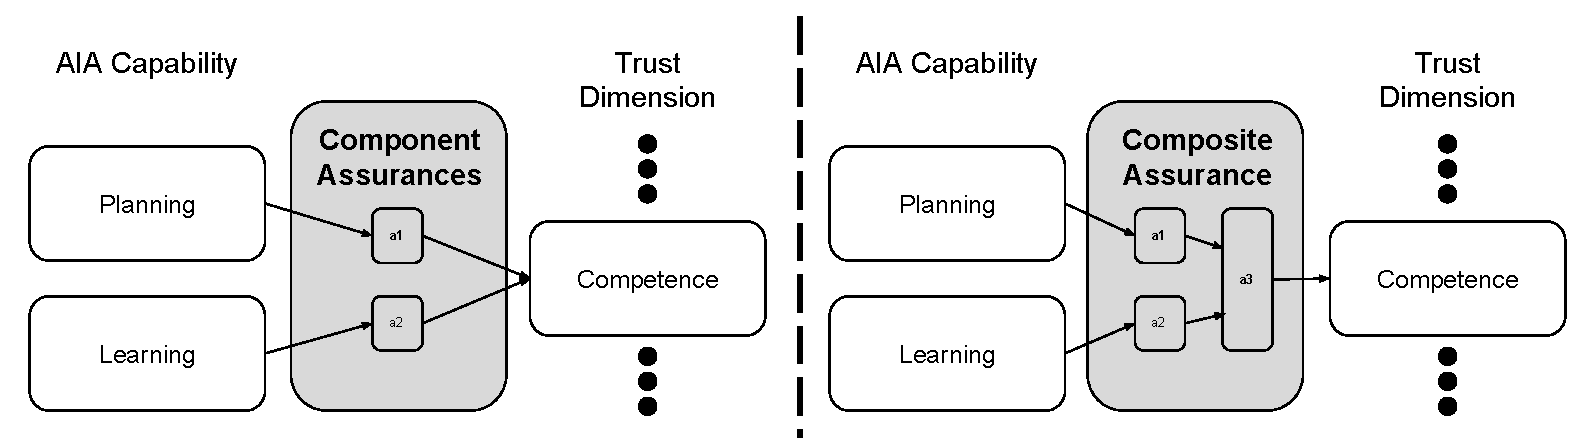
\includegraphics[width=0.9\textwidth]{Figures/Assurance_component_composite.pdf}
    \caption{Figure illustrating the difference between component and composite assurances. The existence of multiple assurances does not imply a composite assurances, rather the combination of multiple component assurances into a single assurance constitutes a composite assurance.}
    \label{fig:assurance_mapping}
\end{figure}

Figure \ref{fig:assurance_mapping} illustrates the concepts of component and composite assurances.

\paragraph{Component Assurances:} Component assurances are perhaps the most well researched in the existing literature. This is likely because several verified component assurances are the predecessors to composite ones. A component assurance might include displaying the confidence of a classification prediction, or visualizing a model as discussed in section \ref{sec:q2}.

\paragraph{Composite Assurances:} Composite assurances are assurances that are built of several components. A notable example is the work by \citet{Aitken2016-cv} who propose a measurement called `self-confidence', applicable to Partially Observable Markov Decision Processes (POMDPs). This metric combines five component assurances into a single composite assurance that is meant to distill the information into a value that a novice operator could understand easily. This paper was discussed in more detail in \ref{sec:q2}. 

    \emph{Tutoring vs Telling:}
Most assurances investigated to date are `telling', in that they do not consider the experience or other traits of different users. The ability to adapt to different users, and to tutor them to appropriate trust will become more critical as time passes due to the diversity of users bases for advanced AIAs and time that users will interact with them. A tutoring assurance would be a planned, dynamic, sequence of assurances that would change in time to adapt to the user's needs. This might include modification of assurances to help a user avoid boredom, or to use the system differently in varying circumstances. It isn't surprising that, to our knowledge, no research has been done with respect to tutoring a user in a trust relationship. This is a complex problem to address that would involve understanding how different users learn, and what an appropriate strategy would be to teach them to have appropriate TRBs. However, a rich resource (not investigated in this paper) would be the work on tutoring systems \citet{Wenger2014-ld} and algorithmic teaching \citet{Balbach2009-jw}.

